\section{Hardware Calibration}
\label{sec:hardware}

The bench calibration tool cls-cal~\cite{clscal} in \oracle{}: measurements of the rack
itself, one page each, laid out as the other tabs (parameters, buttons and result on the
left, plots on the right). Above the pages, \app{Ramp between points} sets the pace of
every unmeasured move, and \app{Line meter: Read (5 $\times$ NPLC 10)} reads the platform
precisely, to check the wiring and polarity against quick tune.

Every measurement drives the DAC by step and confirm, ramps back to 0\,V however it ends,
and writes its record under \code{<data>/hardware\_calibration/} as it goes, so a stopped
or failed one keeps what it took and is analysed as far as it went. On the rack each first
asks the operator to arm the high voltage, naming the most it will apply. \app{Open record...}
shows a record saved earlier, here or on another PC.

\subsection{Settle time}

Steps the platform out and back while the line meter samples on its own timer, and reports
each step's lag, settling and 10--90\,\% rise, overshoot and noise; optionally a \app{Drift
tail} at a long integration. \app{Use as scan settle model} puts the result in force for
scans; \app{Use recommended wait for linearity} sets the sweep's wait to three times the
slowest step (at least 0.2\,s).

\subsection{Linearity}

A count-based ladder up, down, up then down, or in random order (which separates drift from
shape), finer across 0\,V, with 0\,V read again every few rungs and several readings a point
with autozero. It reports gain and offset, residual, curvature, each converter's line and
where they meet 0\,V, hysteresis, the 0\,V drift and, from a dense sweep, each converter's
integral non-linearity. \app{Use as DAC correction} puts a correction in force for
\app{Valid for} days; production runs write uncorrected, since the bench table is applied
after collection, so a correction in force is warned of at every calibration.

\subsection{Cooler monitor}

Streams the cooler meter without gaps, at a short aperture (ripple) or an NPLC (drift), and
reports level, drift, noise by decade, the white-noise floor, the oscillations (mains
harmonics named, corrected for the meter's own attenuation) and the averaged spectrum.

\subsection{Scan table}
\label{sec:table}

The bench table gives the platform voltage each DAC code really gives; each run's
calibration is fitted to it (Section~\ref{sec:calibration}). On the bench tool's records,
the 25 October table predicts the next day's sweep to 11.6\,mV rms once $a + b\,T$ is
fitted.

\begin{description}
    \item[\app{Measure table}] sweeps \app{Span} $\pm$1\,kV (about 1.5\,h) or $\pm$3\,kV
        (about 5\,h, overnight) in 1\,V steps, 5 readings at NPLC 10 a point, 0\,V every 10
        points, \app{Order} up or random, at the Linearity page's settle time and watched
        there. The page warns while the 0\,V checks say the rack is still warming up. The
        sweep is made into a table when it completes.
    \item[\app{Resume...}] takes up a sweep that stopped, from its record, after its last
        0\,V check; the records make one table.
    \item[\app{Check table}] (start of a shift, after a power cycle) reads 250 points across
        the table's span in a few minutes and fits them to it: PASS at 15\,mV rms or less,
        else WARN, measure it again.
    \item[\app{Make from a linearity record...}] builds a table from any sweep with 0\,V
        checks. Tables are kept in \code{<data>/tables/}, named by date and ID (the hash of
        their contents), never overwritten.
    \item[\app{Use a table...}, \app{Compare with...}, \app{Use none}] put one in force, set
        another against it code by code, or use none.
\end{description}

The page shows each converter's shape about a straight line, the 0\,V level's drift and how
often 0\,V should be checked in a run (Figure~\ref{fig:table}). A table from another rack,
or one the settings name that is missing, is warned of at start-up, never refused.

\begin{figure}[ht]
    \centering
    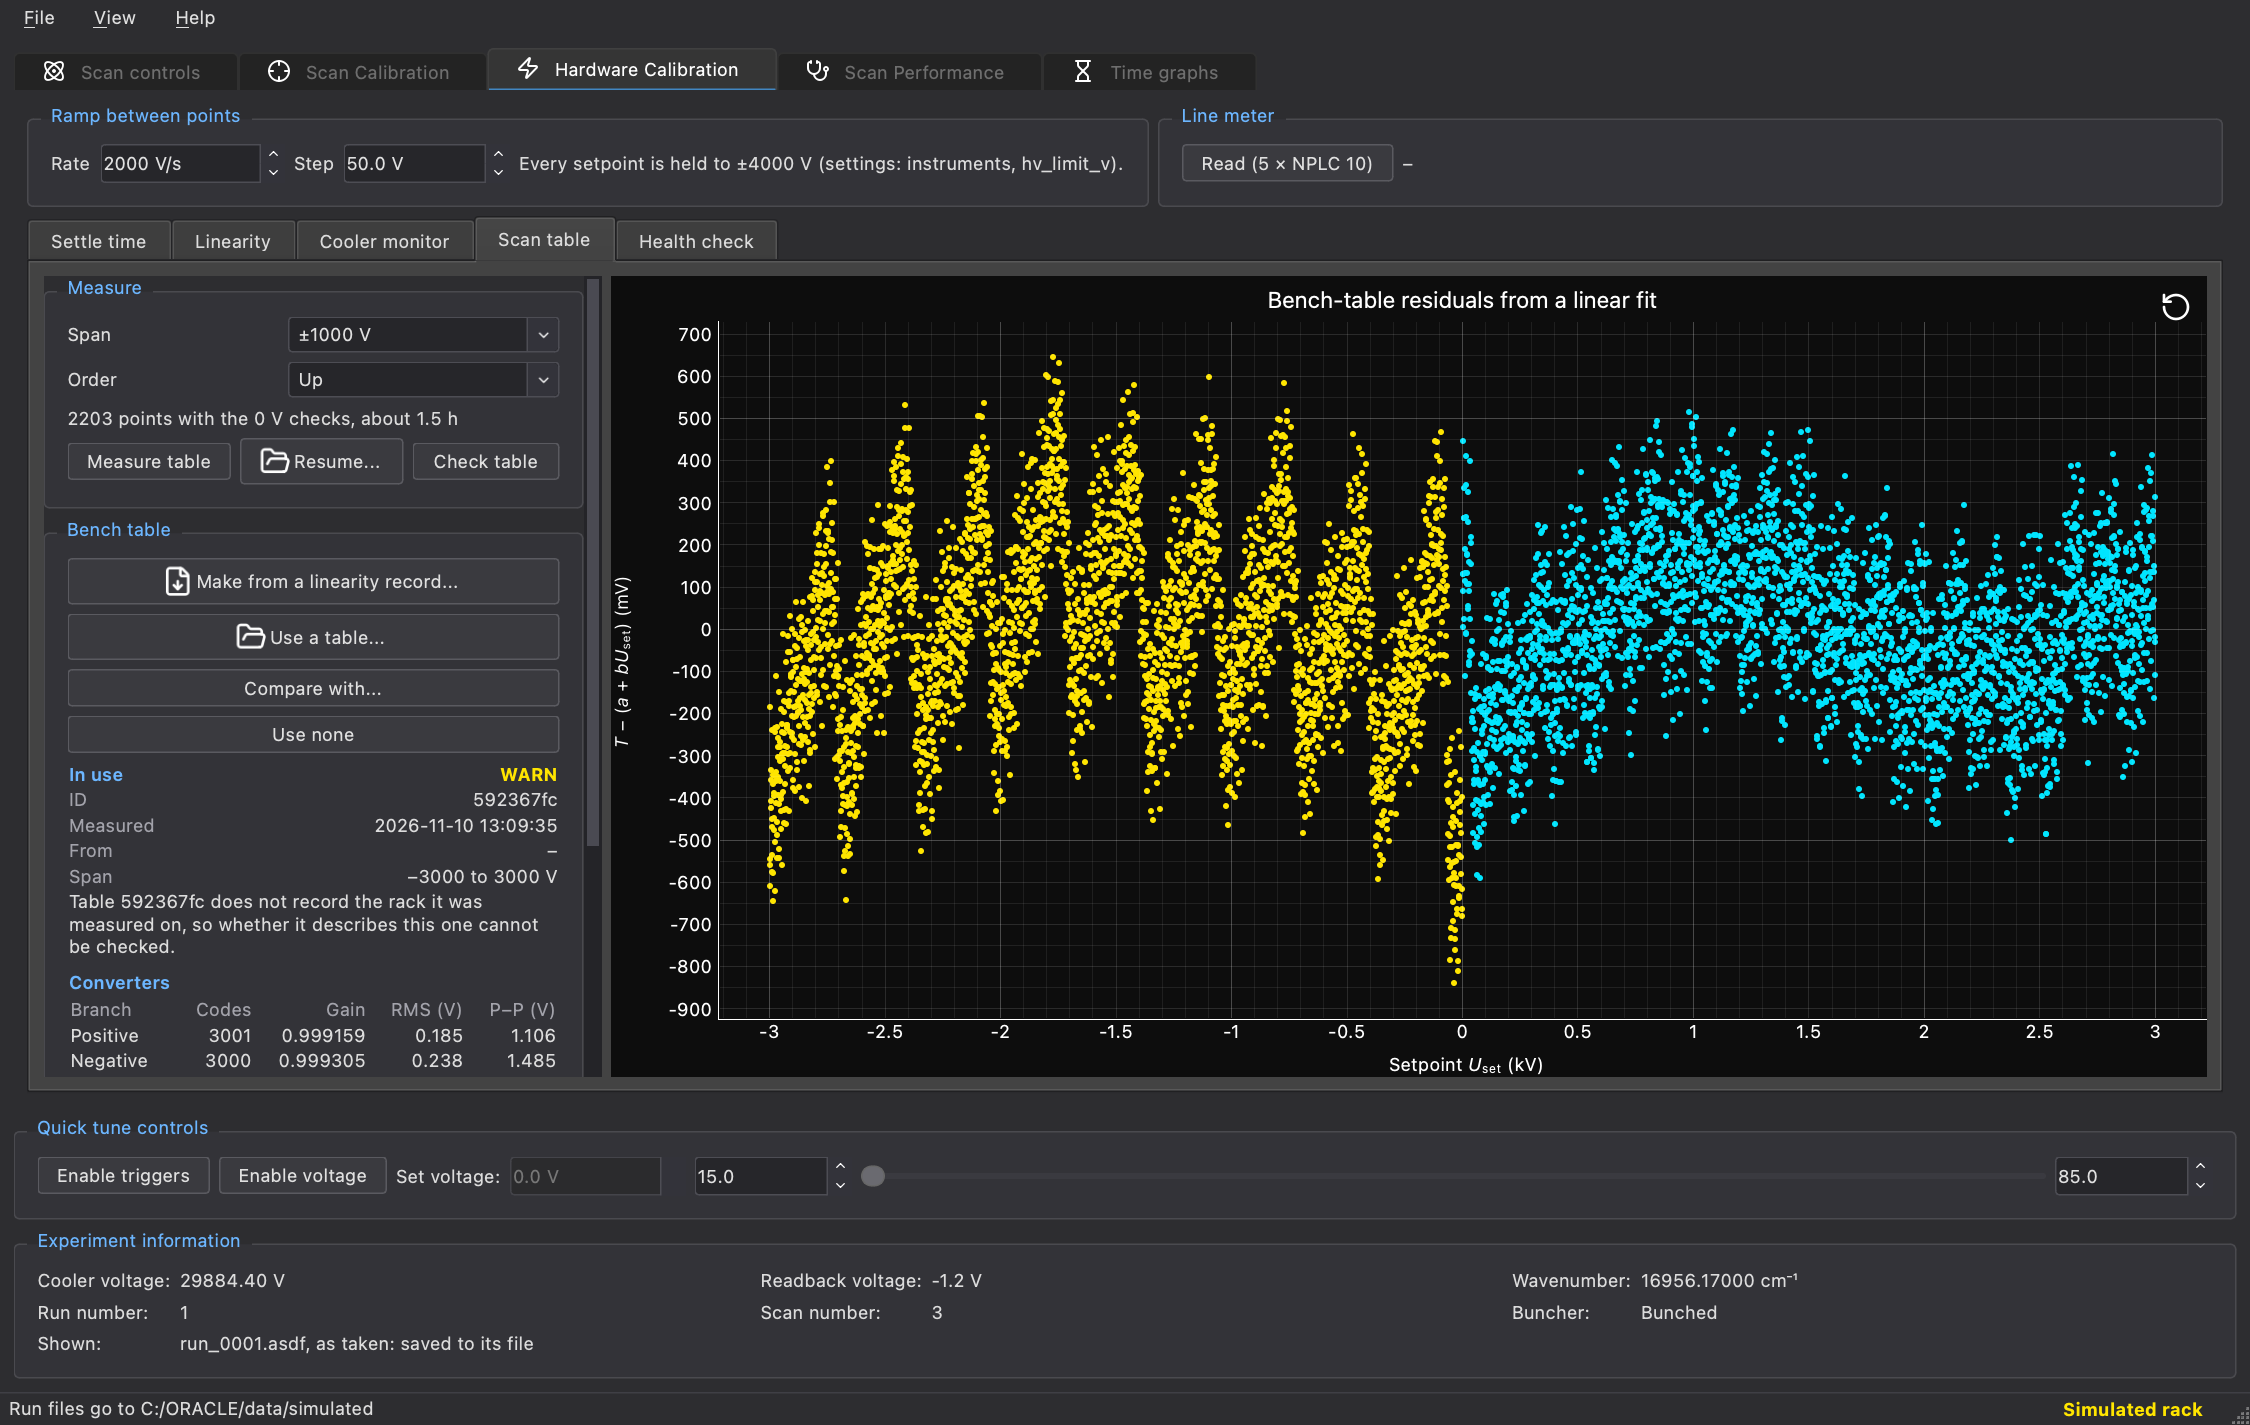
\includegraphics[width=\textwidth]{fig_hardware_table}
    \caption{The \app{Scan table} page with the 25 October 2026 bench table in force: each
        converter's residual from a straight line.}
    \label{fig:table}
\end{figure}

\subsection{Health check}

One report, at the start of a shift, on whether the rack is as it should be
(Figure~\ref{fig:health}). With \app{Check the bench table first} and a table in force it
runs the table check; then it reads the cooler for 10\,s (its 50\,Hz ripple), runs the Scan
tab's triggers for 10\,s counting each PMT (with the beam off, its dark counts) and the
triggers, and reads both meters' trigger sources. Each part is set against the last check:
WARN for ripple grown by half, a PMT silent or changed more than twice over, a trigger
miscounted or lost, or a meter on its trigger input. Every check is kept as
\code{hardware\_calibration/health\_<time>.yaml}; \app{Post to ELOG} posts it.

\begin{figure}[ht]
    \centering
    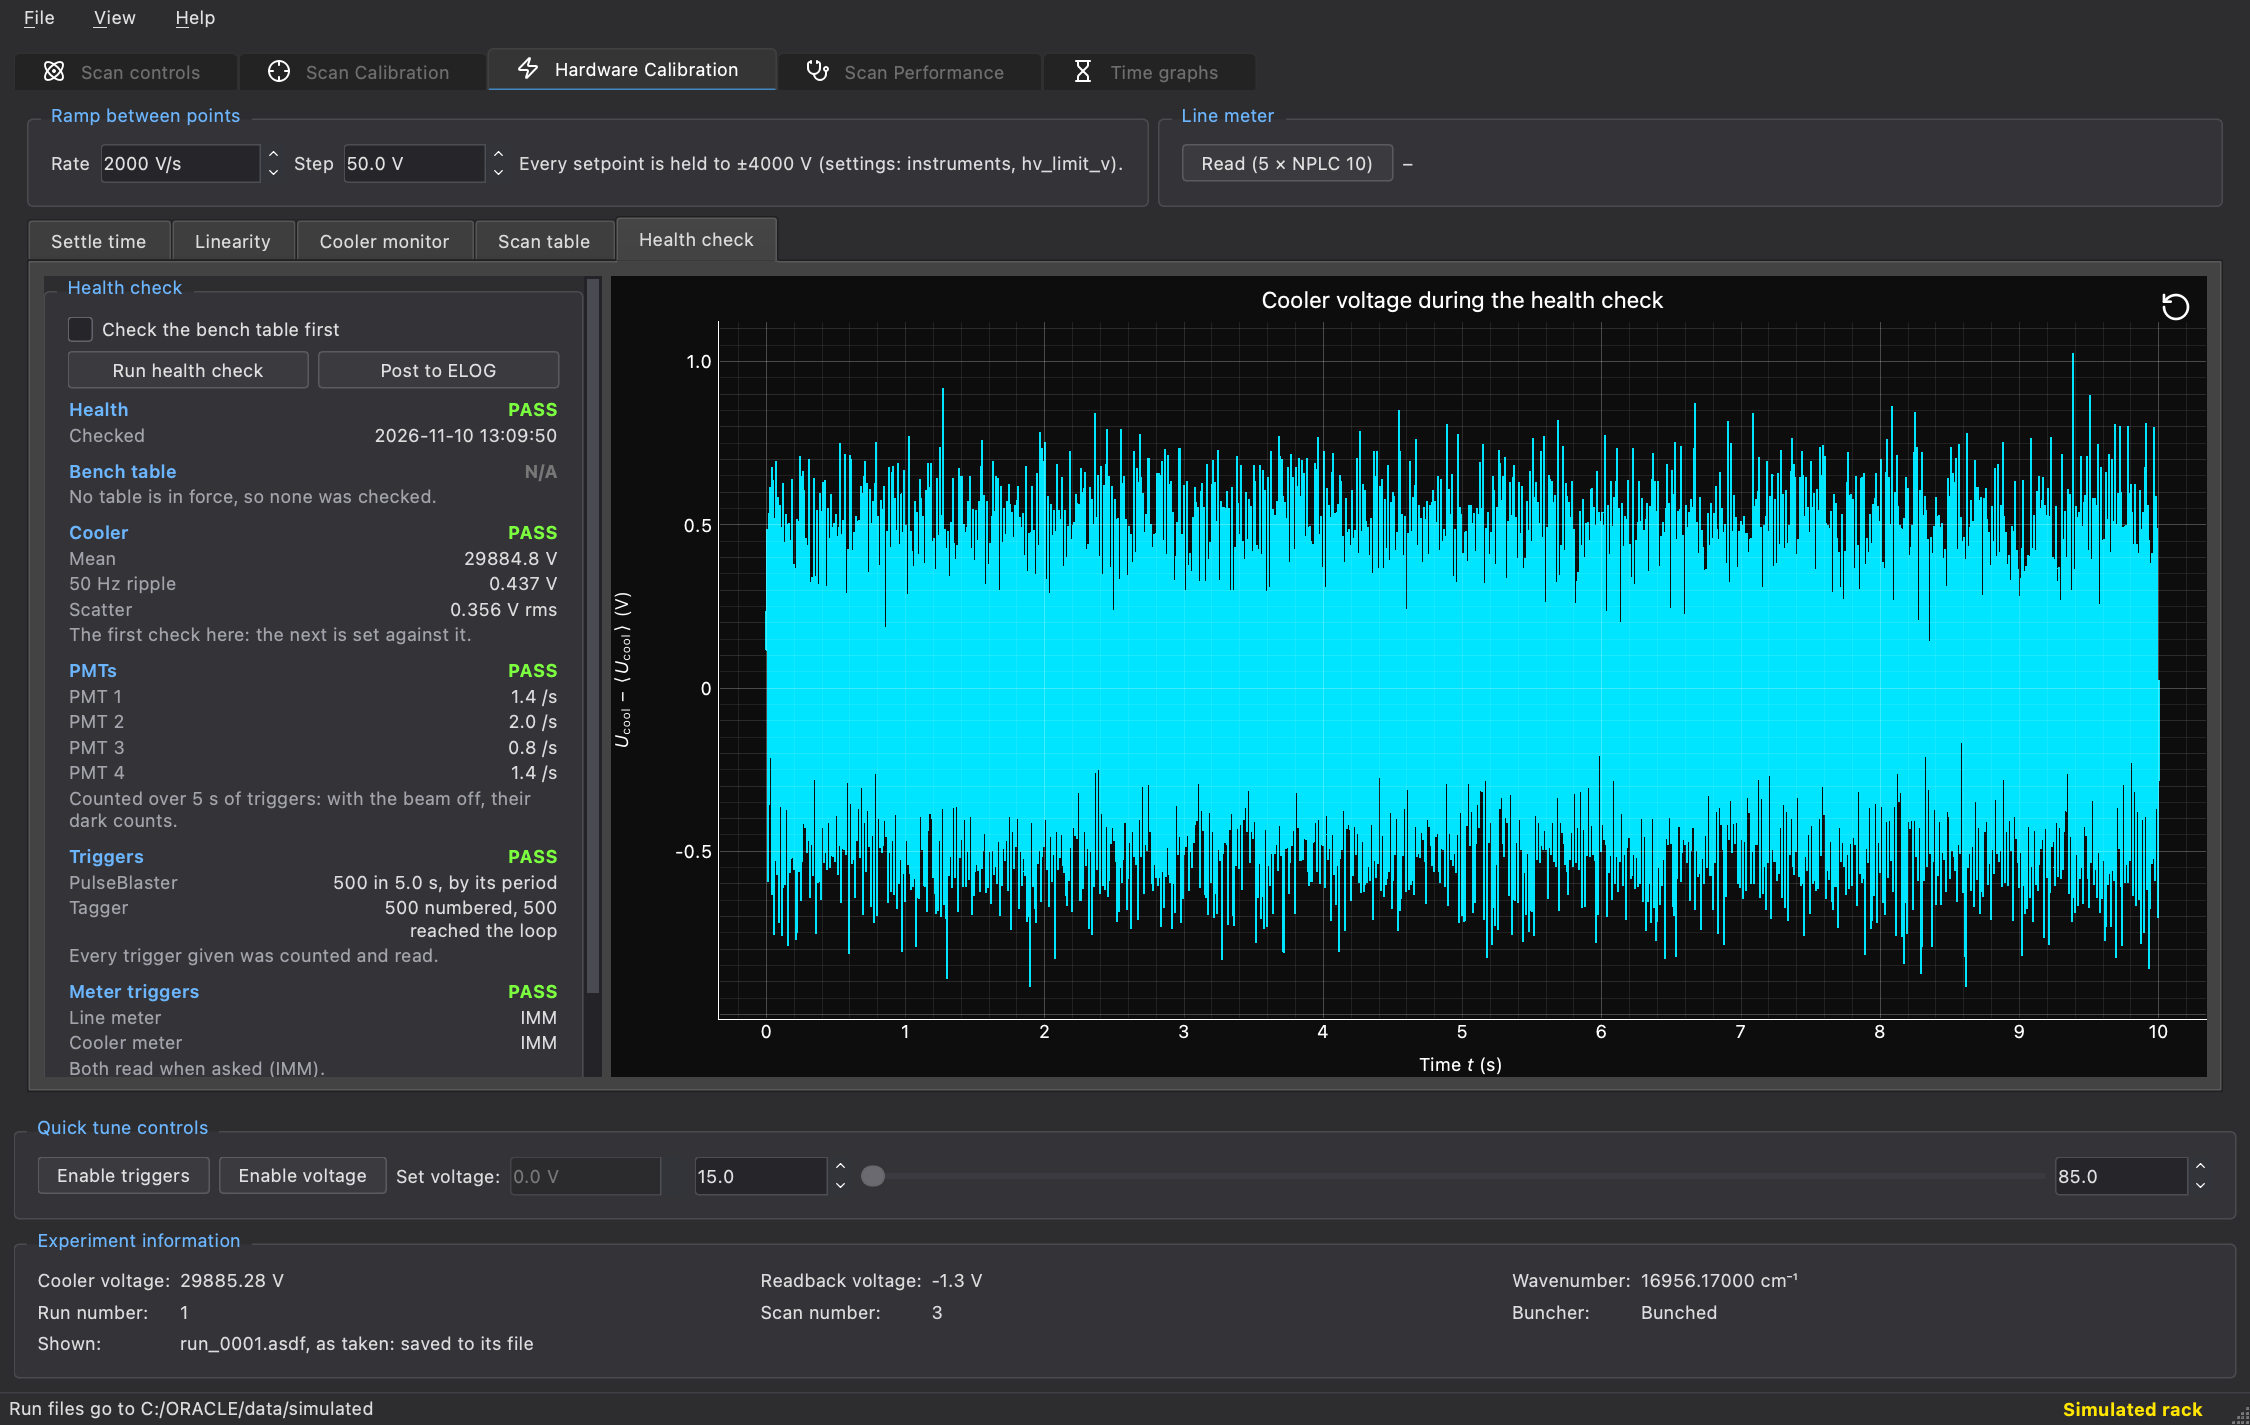
\includegraphics[width=\textwidth]{fig_health_check}
    \caption{A health check on the simulated rack, and the cooler it read.}
    \label{fig:health}
\end{figure}
